\scanpage{103}\deleted{\unsure{93|95}}\mspage{94.}
Cas où on ne fait pas l'hyp. par exemple
% slanted
\margin{\uline{\unsure{Cancelé|Cancellé|Calculé}}}
\diagram{\begin{tikzcd}[ampersand replacement=\&,row sep=small,column sep=small]
 \& b \&\\
 a\arrow[ur,line width=.95pt] \& \& \unsure{c|e}\arrow[ul]
\end{tikzcd}}
\[
\begin{aligned}
 \mathrm{cosupp}^{\circ}(\{P_a\})&=\{P_b\unsure{\}}\unsure{,|;}\\
 \mathrm{supp}^{\circ}(\{P_a\})&=\{P_a,P_{\unsure{c|b}},\inserted{\deleted{\unsure{P}}\unsure{S|P}_{ab},S_{c,b}}\}\ne\{P_a\}
\end{aligned}
\]
\[
 \unsure{\downarrow|J}=\mathrm{cosupp}^{\circ}(P_b)=\unsure{M|\mathcal M}\setminus\{P_b\}
\]
\[
\begin{aligned}
 \mathrm{cosupp}^{\circ}(\deleted{\unsure{\{P_a\}}}\widetilde{S_{ab}})&=\varnothing\\
 \mathrm{supp}^{\circ}(\widetilde{S_{ab}})&=M\ne\mathrm{Omb}(S_{ab})
\end{aligned}
\]
(NB $M=\mathrm{Omb}(S_{ab})\amalg\{S_{c,b},P_c\}$

ici $\mathrm{card}\,M=5$

Par contre, pas de Pb avec
\diagram{\begin{tikzcd}[ampersand replacement=\&,row sep=small,column sep=small]
 \& b \&\\
 a\arrow[ur] \& \& d\arrow[ul]\\
 \& c\arrow[ul]\arrow[ur] \&
\end{tikzcd}}
p. ex.

\[
\begin{aligned}
 &\deleted{\mathrm{cosupp}^{\circ}P_a=\{P_b,P_c\},S_{ab},S_{ca}\}}\\
 &\deleted{\mathrm{supp}^{\circ}P_a=}
\end{aligned}
\]
\deleted{\uline{Lemme 2} Soient} $\deleted{\Phi\subset M,\ \Psi\subset M\ \unsure{t}}$ \deleted{$X,Y\in M$ avec $X\parallel Y$, et soit $\Phi\subset\mathrm{Omb}(X)$,} $\deleted{\unsure{\Psi}}$ \deleted{($=\mathrm{supp}\,\widetilde X$ par lemme 1), $\Psi\subset\mathrm{Omb}(Y)$ ($=\mathrm{supp}\,\widetilde Y$). Alors}
\[
 \deleted{\mathrm{supp}^{\circ}(\Phi\cup\Psi)=\mathrm{supp}^{\circ}\Phi\cup\mathrm{supp}^{\circ}\Psi.}
\]

% slanted
\margin{4 \uline{juillet}}
Détermination des \unsure{préfigures|profigures}, ou ensembles constructibles \unsure{dans|de ce|de} $M$.

\deleted{Les} Pour la relation d'ordre induite, une préfigure se décompose en composantes connexes. Les composantes connexes \inserted{(ou préfigures connexes)} sont des types \unsure{suivant|suivants} 

\deleted{a) Dim 0}
\figure{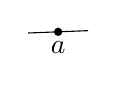
\begin{tikzpicture}[baseline]\fill (0,0) circle (1.5pt) node[below] {$\deleted{a}$};
\draw (-.38,-.015)--(.38,.015);\end{tikzpicture}}
\deleted{$\Phi=\{P_a\}$ c'est une figure \unsure{fermée|ferm}}

\deleted{b) Dim 1\qquad b) Figure}
\figure{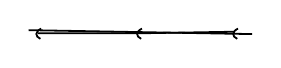
\begin{tikzpicture}[line width=.65pt]\draw (0,0)--(1.28,0)--(2.5,.02);
\foreach \x in {0,1.28,2.5}{\draw (\x+.04,.06) .. controls (\x-.04,.02) and (\x-.04,-.04) .. (\x+.03,-.07);}
\draw (-.12,.04)--(2.72,-.01);\end{tikzpicture}}
% archive sheet number: 103
